\documentclass[10pt]{article}
\usepackage{../pplmanual,pst-node}
\input{../pplmanual}

\title{Adaptive MPI Manual}
\version{1.0}
\credits{
AMPI was originally developed by Milind Bhandarkar with inputs from Gengbin Zheng and
Orion Lawlor at the parallel programming lab at the University of Illinois. 
The derived data types (DDT) library, which AMPI uses for the 
derived data types support, has been developed by Neelam Saboo.
}

\begin{document}
\maketitle

\section{Introduction}

This manual describes Adaptive MPI~(\ampi{}), which is an implementation of the
MPI standard\footnote{Currently, AMPI supports the MPI-2.2 standard, and the MPI-3.1 standard is under active development,
though we already support non-blocking and neighborhood collectives among other MPI-3.1 features.} on top of \charmpp{}.
\ampi{} acts as a regular MPI implementation (akin to MPICH, OpenMPI, MVAPICH, etc.)
with several built-in extensions that allow MPI developers to take advantage of \charmpp{}'s
dynamic runtime system, which provides support for process virtualization,
overlap of communication and computation, load balancing, and fault tolerance
with zero to minimal changes to existing MPI codes.

In this manual, we first describe the philosophy behind Adaptive MPI, then give a brief
introduction to \charmpp{} and rationale for \ampi{}. We then describe
\ampi{} in detail. Finally we summarize the changes required for existing MPI
codes to run with \ampi{}. Appendices contain the details of installing
\ampi{}, and building and running \ampi{} programs.

\subsection{Overview}

Developing parallel Computational Science and Engineering (CSE) applications is
a complex task. One has to implement the right physics, develop or choose and
code appropriate numerical methods, decide and implement the proper input and
output data formats, perform visualizations, and be concerned with correctness
and efficiency of the programs. It becomes even more complex for multi-physics
coupled simulations, many of which are dynamic and adaptively refined 
so that load imbalance becomes a major challenge. In addition to imbalance
caused by dynamic program behavior, hardware factors such as latencies,
variability, and failures must be tolerated by applications.
Our philosophy is to lessen the burden of application developers by
providing advanced programming paradigms and versatile runtime systems that can
handle many common programming and performance concerns automatically and let
application programmers focus on the actual application content.

Many of these concerns can be addressed using the processor virtualization and 
over-decomposition philosophy of \charmpp{}. Thus, the developer only sees 
virtual processors and lets the runtime system deal with underlying physical 
processors. This is implemented in \ampi{} by mapping MPI ranks to \charmpp{}
user-level threads as illustrated in Figure\ref{fig_virt}. As an immediate and
simple benefit, the programmer can use as many virtual processors ("MPI ranks")
as the problem can be easily decomposed to. For example, suppose the problem
domain has $n*2^n$ parts that can be easily distributed but programming for
general number of MPI processes is burdensome, then the developer can have
$n*2^n$ virtual processors on any number of physical ones using \ampi{}.
  
\begin{figure}[h]
\centering
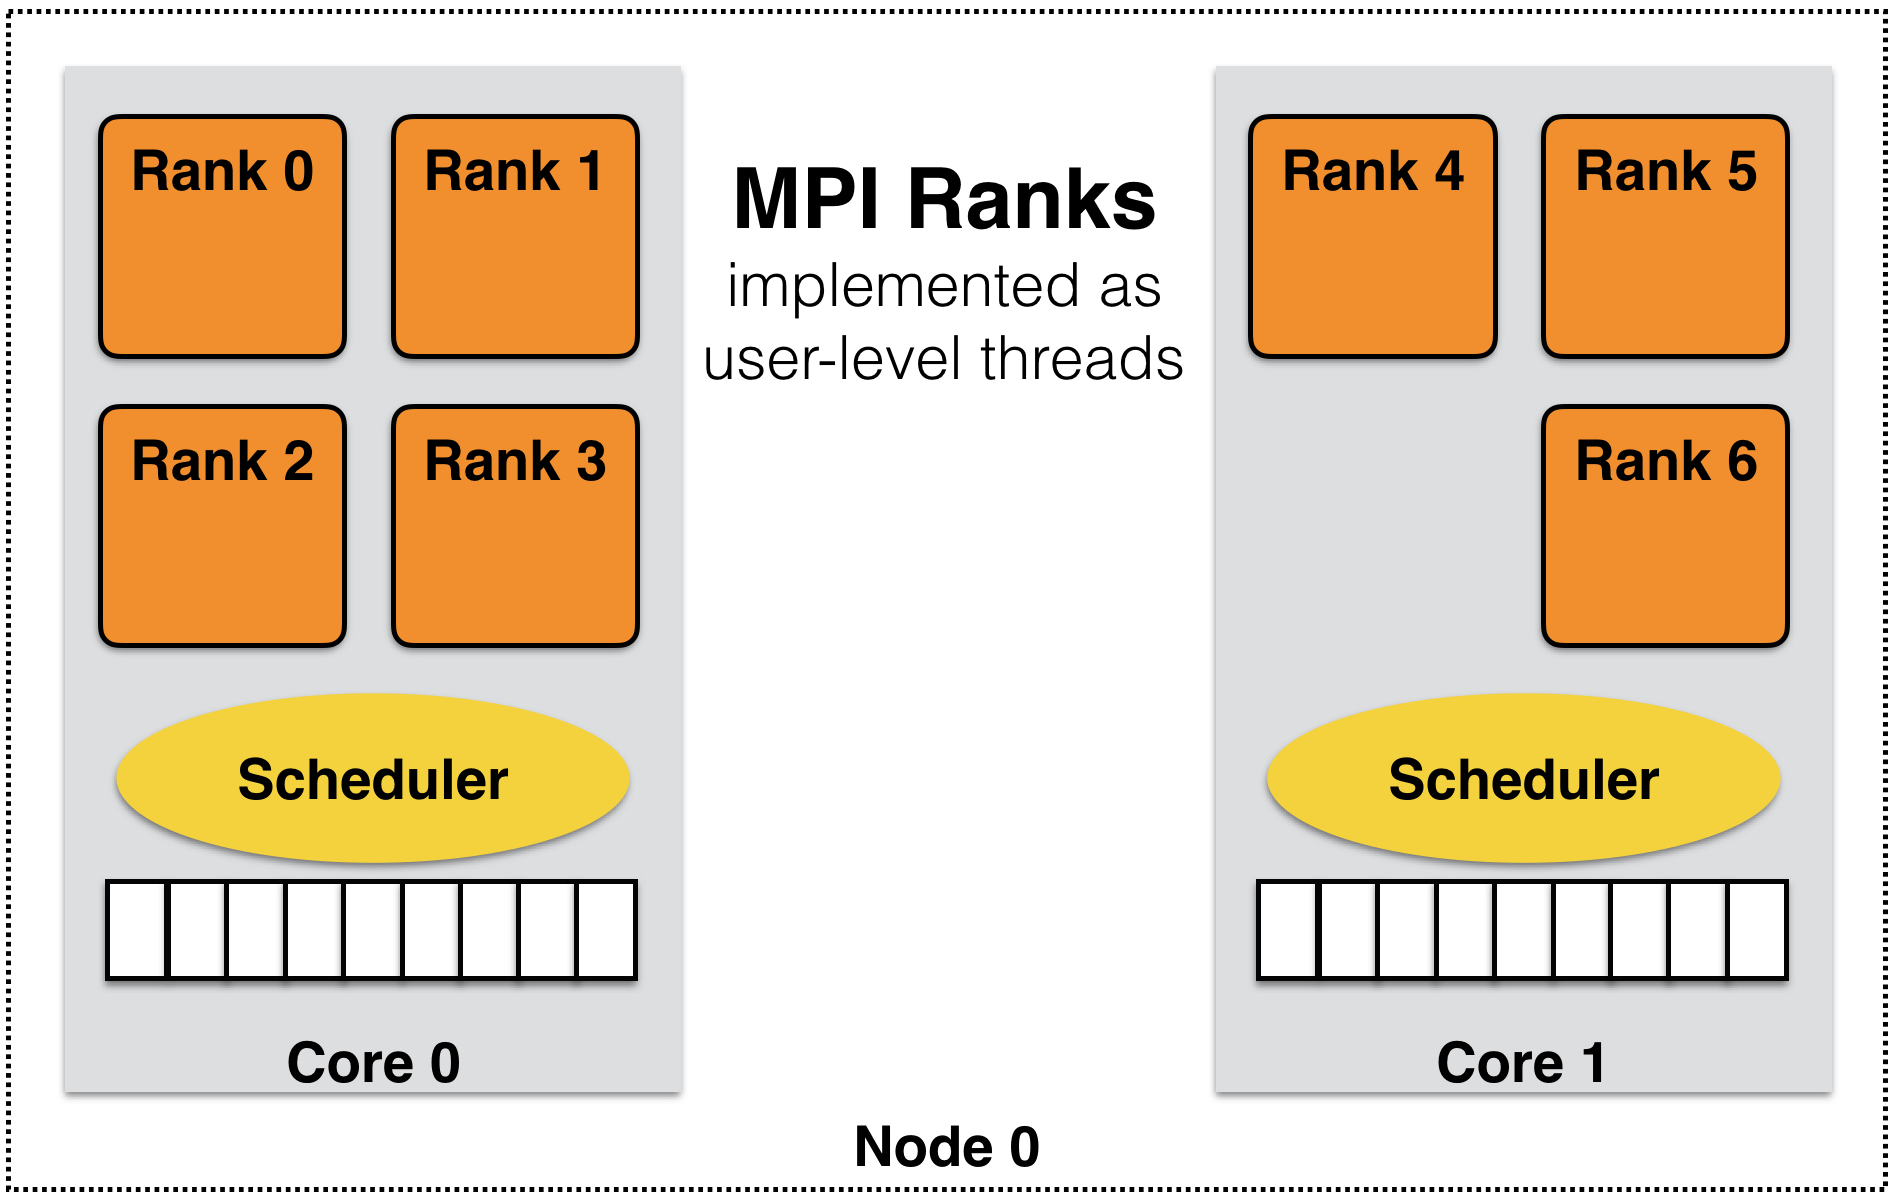
\includegraphics[width=4.6in]{figs/virtualization.png}
\caption{MPI ranks are implemented as user-level threads in \ampi{} rather than Operating System processes.}
\label{fig_virt}
\end{figure}

\ampi{}'s execution model consists of multiple user-level threads per Processing Element (PE).
The \charmpp{} scheduler coordinates
execution of these user-level threads (also called Virtual Processors or VPs) and controls
execution. These VPs can also migrate between
PEs for the purpose of load balancing or other reasons. The number of VPs
per PE specifies the virtualization ratio (degree of over-decomposition).
For example, in Figure \ref{fig_virt} the virtualization ratio is $3.5$ (there are
four VPs on PE 0 and three VPs on PE 1). Figure \ref{fig_prac} show how the problem domain
can be over-decomposed in \ampi{}'s VPs as opposed to other MPI implementations.

\begin{figure}[h]
\centering
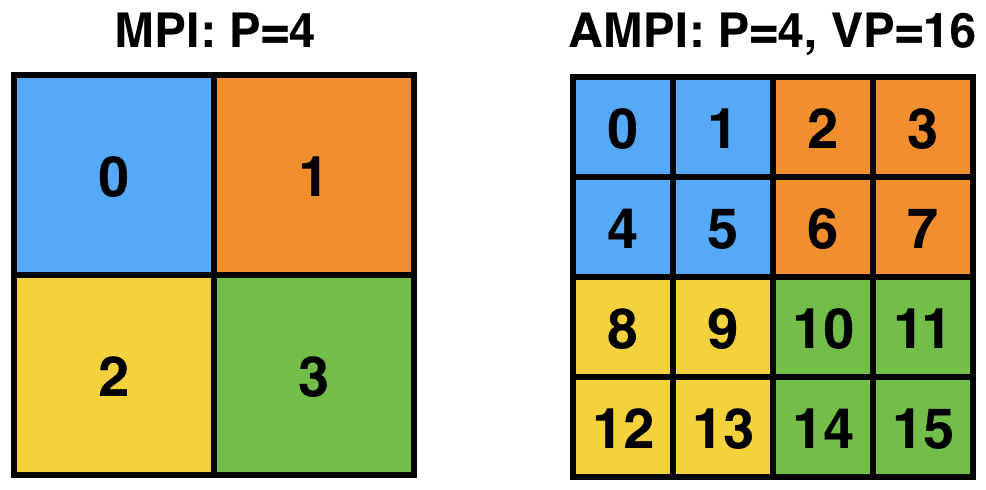
\includegraphics[width=4.6in]{figs/prac.png}
\caption{The problem domain is over-decomposed to more VPs than PEs.}
\label{fig_prac}
\end{figure}

Another benefit of virtualization is communication and computation overlap, which
is automatically realized in \ampi{} without programming effort.
Techniques such as software pipelining require significant programming
effort to achieve this goal and improve performance. However, one can use \ampi{}
to have more virtual processors than physical processors to overlap communication
and computation. Each time a VP is blocked for communication, the \charmpp{}
scheduler picks the next VP among those that are ready to execute. In this
manner, while some of the VPs of a physical processor are waiting for a message
to arrive, others can continue their execution. Thus, performance improves
without any changes to the application source code.

Another potential benefit is that of better cache utilization. With
over-decomposition, a smaller subdomain is accessed by a VP repeatedly
in different function calls before getting blocked by communication and
switching to another VP. That smaller subdomain may fit into cache if
over-decomposition is enough. This concept is illustrated in Figure
\ref{fig_virt} where each \ampi{} rank's subdomain is smaller than the
corresponding MPI subdomain and so may fit into cache memory. Thus,
there is a potential performance improvement without changing the source code.

One important concern is that of load imbalance. New generation parallel
applications are dynamically varying, meaning that processors' load is
shifting during execution. In a dynamic simulation application such as
rocket simulation, burning solid fuel, sub-scaling for a certain part of
the mesh, crack propagation, particle flows all contribute to load imbalance.
A centralized load balancing strategy built into an application is
impractical since each individual module is developed mostly independently by
various developers. In addition, embedding a load balancing strategy in the code
complicates it greatly, and programming effort increases significantly. The
runtime system is uniquely positioned to deal with load imbalance. Figure
\ref{fig_migrate} shows the runtime system migrating a VP after detecting
load imbalance. This domain may correspond to a weather forecast model
where there is a storm cell in the top-left quadrant, which requires more
computation to simulate. \ampi{} will then migrate VP 1 to balance the
division of work across processors and improve performance. Note that
incorporating this sort of load balancing inside the application code may
take a lot of effort and complicate the code.

\begin{figure}[h]
\centering
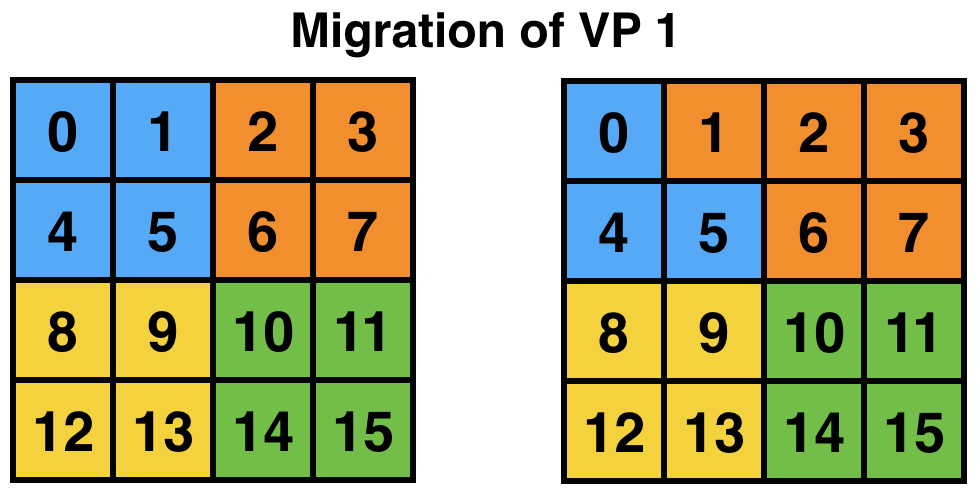
\includegraphics[width=4.6in]{figs/migrate.png}
\caption{\ampi{} can migrate VPs across processes for load balancing.}
\label{fig_migrate}
\end{figure}

There are many different load balancing strategies built into \charmpp{} that
can be selected by an \ampi{} application developer. Among those, some may
fit better for a particular application depending on its characteristics.
Moreover, one can write a new load balancer, best suited for an application,
by the simple API provided inside \charmpp{} infrastructure.
Our approach is based on actual measurement of load information at runtime,
and on migrating computations from heavily loaded to lightly loaded processors.

For this approach to be effective, we need the computation to be split into
pieces many more in number than available processors. This allows us to
flexibly map and re-map these computational pieces to available processors.
This approach is usually called "multi-domain decomposition".

\charmpp{}, which we use as a runtime system layer for the work described here,
simplifies our approach. It embeds an elaborate performance tracing mechanism,
a suite of plug-in load balancing strategies, infrastructure for defining and
migrating computational load, and is interoperable with other programming
paradigms.


\section{\charmpp{}}

\charmpp{} is an object-oriented parallel programming library for \CC{}.  It
differs from traditional message passing programming libraries (such as MPI) in
that \charmpp{} is "message-driven". Message-driven parallel programs do not
block the processor waiting for a message to be received.  Instead, each
message carries with itself a computation that the processor performs on
arrival of that message. The underlying runtime system of \charmpp{} is called
\converse{}, which implements a "scheduler" that chooses which message to
schedule next (message-scheduling in \charmpp{} involves locating the object
for which the message is intended, and executing the computation specified in
the incoming message on that object). A parallel object in \charmpp{} is a
\CC{} object on which a certain computations can be asked to be performed from
remote processors.

\charmpp{} programs exhibit latency tolerance since the scheduler always picks
up the next available message rather than waiting for a particular message to
arrive.  They also tend to be modular, because of their object-based nature.
Most importantly, \charmpp{} programs can be \emph{dynamically load balanced},
because the messages are directed at objects and not at processors; thus
allowing the runtime system to migrate the objects from heavily loaded
processors to lightly loaded processors.

Since many CSE applications are originally written using MPI, one would have to
rewrite existing code if they were to be converted to \charmpp{} to take
advantage of dynamic load balancing and other \charmpp{} features. This is
indeed impractical. However, \converse{} -- the runtime system of \charmpp{} --
supports interoperability between different parallel programming paradigms
such as parallel objects and threads. Using this feature, we developed
\ampi{}, which is described in more detail in the next section.

\section{AMPI}

\ampi{} utilizes the dynamic load balancing and other capabilities of \charmpp{} by
associating a "user-level" thread with each \charmpp{} migratable object.
User's code runs inside this thread, so that it can issue blocking receive
calls similar to MPI, and still present the underlying scheduler an opportunity
to schedule other computations on the same processor. The runtime system keeps
track of the computational loads of each thread as well as the communication graph
between \ampi{} threads, and can migrate these threads in order to balance the
overall load while simultaneously minimizing communication overhead.

\subsection{AMPI Compliance to MPI Standards}

Currently \ampi{} supports the MPI-2.2 standard, with preliminary support for most MPI-3.1
features and a collection of extensions explained in detail in this manual. One-sided
communication calls in MPI-2 and MPI-3 are implemented, but they do not yet
take advantage of RMA features. Non-blocking collectives have been defined in
\ampi{} since before MPI-3.0's adoption of them. Also
ROMIO\footnote{http://www-unix.mcs.anl.gov/romio/} has been integrated into
\ampi{} to support parallel I/O features.

\subsection{AMPI Extensions to MPI Standards}

The following are AMPI extensions to the MPI standard, which will be explained in
detail in this manual. All AMPI extensions to the MPI standard are prefixed with
\texttt{AMPI\_} rather than \texttt{MPI\_}. All extensions are available in C, C++, and Fortran,
with the exception of \texttt{AMPI\_Command\_argument\_count} and
\texttt{AMPI\_Get\_command\_argument} which are only available in Fortran.

\begin{alltt}
AMPI_Migrate          AMPI_Register_pup            AMPI_Get_pup_data
AMPI_Migrate_to_pe    AMPI_Set_migratable          AMPI_Evacuate
AMPI_Load_set_value   AMPI_Load_start_measure      AMPI_Load_stop_measure
AMPI_Iget             AMPI_Iget_wait               AMPI_Iget_data
AMPI_Iget_free        AMPI_Type_is_contiguous      AMPI_Register_main
AMPI_Yield            AMPI_Suspend                 AMPI_Resume
AMPI_Alltoall_medium  AMPI_Alltoall_long
AMPI_Register_just_migrated         AMPI_Register_about_to_migrate
AMPI_Command_argument_count         AMPI_Get_command_argument
\end{alltt}

\ampi{} provides a set of built-in attributes on all communicators and windows
to find the number of the worker thread, process, or host that a rank is currently running on,
as well as the total number of worker threads, processes, and hosts in the job.
We define a worker thread to be a thread on which one of more \ampi{} ranks are scheduled.
We define a process here as an operating system process, which may contain one or more
worker threads. The built-in attributes are \texttt{AMPI\_MY\_WTH}, \texttt{AMPI\_MY\_PROCESS},
\texttt{AMPI\_NUM\_WTHS}, and \texttt{AMPI\_NUM\_PROCESSES}. These attributes are
accessible from any rank by calling \texttt{MPI\_Comm\_get\_attr}, such as:

\begin{alltt}
! Fortran:
integer :: my_wth, flag, ierr
call MPI_Comm_get_attr(MPI_COMM_WORLD, AMPI_MY_WTH, my_wth, flag, ierr)

// C/C++:
int my_wth, flag;
MPI_Comm_get_attr(MPI_COMM_WORLD, AMPI_MY_WTH, &my_wth, &flag);
\end{alltt}

\ampi{} also provides extra communicator types that users can pass to
\texttt{MPI\_Comm\_split\_type}: \texttt{AMPI\_COMM\_TYPE\_HOST} for splitting a communicator into
disjoint sets of ranks that share the same physical host, \texttt{AMPI\_COMM\_TYPE\_PROCESS} for
splitting a communicator into disjoint sets of ranks that share the same operating system process,
and \texttt{AMPI\_COMM\_TYPE\_WTH}, for splitting a communicator into disjoint sets
of ranks that share the same worker thread.

For parsing Fortran command line arguments, AMPI Fortran programs should use
our extension APIs, which are similar to Fortran 2003's standard APIs. For example:

\begin{alltt}
integer :: i, argc, ierr
integer, parameter :: arg_len = 128
character(len=arg_len), dimension(:), allocatable :: raw_arguments

call AMPI_Command_argument_count(argc)
allocate(raw_arguments(argc))
do i = 1, size(raw_arguments)
    call AMPI_Get_command_argument(i, raw_arguments(i), arg_len, ierr)
end do
\end{alltt}

\subsection{Name for Main Program}

To convert an existing program to use AMPI, the main function or program
may need to be renamed. The changes should be made as follows:

\subsubsection{Fortran}

You must declare the main program as a subroutine called "MPI\_MAIN". 
Do not declare the main subroutine as a \textit{program} because 
it will never be called by the AMPI runtime.

\begin{alltt}

program pgm -> subroutine MPI_Main
	...		    		      ...
end program -> end subroutine
\end{alltt}

\subsubsection{C or C++}

The main function can be left as is, if \texttt{mpi.h} is included before the main function. 
This header file has a preprocessor macro that renames main, and 
the renamed version is called by the AMPI runtime by each thread.


\subsection{Global Variable Privatization}

For the before-mentioned benefits to be effective, one needs to map multiple
user-level threads onto each processor. Traditional MPI programs assume that the
entire processor is allocated to themselves, and that only one thread of
control exists within the process's address space. So, they may safely use global and
static variables in the program. However, global and static variables are
problematic for multi-threaded environments such as \ampi{} or OpenMP.
This is because there is a single instance of those variables so they will be 
shared among different threads in the single address space, so if programmers are not careful
a wrong result may be produced by the program.
Figure \ref{fig_global} shows an example of a multi-threaded application with 
two threads in a single process. $var$ is a global or static variable in this 
example. Thread 1 assigns a value to it, then it gets blocked for communication 
and another thread can continue. Thereby, thread 2 is scheduled next and 
accesses $var$ which is wrong. The semantics of this program needs separate
instances of $var$ for each of the threads. That is where the need arises
to make some transformations to the original MPI program in order to run
correctly with \ampi{}. Note, this is the only change necessary to run an MPI 
program with \ampi{}, that the program be thread-safe and have no global or static
variables whose values differ across different MPI ranks. Also note that global variables
that are constant or are only written to once to the same value across all ranks
during initialization are already thread-safe.

\begin{figure}[h]
\centering
\includegraphics[width=4.6in]{figs/global.png}
\caption{Mutable global or static variables are an issue for \ampi{}}
\label{fig_global}
\end{figure}

The basic transformation needed to port the MPI program to \ampi{} is
privatization of global variables.
With the MPI process model, each MPI node can keep a copy of its own
"permanent variables" -- variables that are accessible from more than one
subroutines without passing them as arguments.  Module variables, "saved"
subroutine local variables, and common blocks in Fortran90 belong to this
category. If such a program is executed without privatization on \ampi{}, all
the \ampi{} threads that reside in the same process will access the same copy of
such variables, which is clearly not the desired semantics.  To ensure correct
execution of the original source program, it is necessary to make such
variables "private" to individual threads. We provide three choices with varying
degrees of developer effort required and varying degrees of portability:
manual encapsulation of global state, a thread-local storage based automated mechanism, and
global offset table based automated mechanism.

\subsubsection{Automatic Thread-Local Storage Swapping}
Thread Local Store (TLS) was originally employed in kernel threads to
localize variables and provide thread safety. It can be used by annotating
global/static variable declarations in \CC{} with \emph{thread\_local}
and in C with \emph{\_\_thread}. Thus, those variables will have one instance
per extant thread. This keyword is not an official extension of the C language,
though compiler writers are encouraged to implement this feature. Currently,
the ELF object file format supports Thread Local Storage.

It handles both global and static variables and has no context-switching
overhead. AMPI provides runtime support for privatizing thread-local variables to user-level threads
by changing the TLS segment register when context switching between user-level threads.
Currently, \charmpp{} supports it for x86/x86\_64 platforms when using GNU compilers.

For the example above, the following changes to the code handle the global variables:
\begin{alltt}
thread_local int myrank;
thread_local double xyz[100];
\end{alltt}

The runtime system also should know that TLS-Globals is used at both compile and link time:

\begin{alltt}
ampicxx -o example example.C -tlsglobals
\end{alltt}

\subsubsection{Automatic Global Offset Table Swapping}
Thanks to the ELF Object Format, we have successfully automated the procedure 
of switching the set of user global variables when switching thread contexts.
Executable and Linkable Format (ELF) is a common standard file format 
for Object Files in Unix-like operating systems.
ELF maintains a Global Offset Table (GOT) for globals so it is possible to
switch GOT contents at thread context-switch by the runtime system.

The only thing that the user needs to do is pass the flag {\tt -swapglobals}
at both compile and link time (e.g. "ampicc -o prog prog.c -swapglobals"). This method does not require
any changes to the source code and works with any language (C, C++, Fortran, etc).
However, it does not handle static variables, has a context switching
overhead that grows with the number of global variables, and is incompatible with SMP builds
of AMPI, where multiple virtual ranks can execute simulataneously on different scheduler threads
within an OS process.
Currently, this feature only works on x86 and x86\_64 platforms that fully support ELF,
and it requires ld version 2.23 or older, or else a patched version of ld 2.24+ that we provide
here: https://charm.cs.illinois.edu/gerrit/gitweb?p=libbfd-patches.git;a=tree;f=swapglobals

\subsubsection{Manual Change}
We have employed a strategy of argument passing to do this privatization
transformation. That is, the global variables are bunched together in a
single user-defined type, which is allocated by each thread dynamically or on the stack.
Then a pointer to this type is passed from subroutine to subroutine as an argument.
Since the subroutine arguments are passed on the stack, which is not shared
across all threads, each subroutine when executing within a thread operates on
a private copy of the global variables. 

This scheme is demonstrated in the following examples. The original Fortran90
code contains a module \texttt{shareddata}. This module is used in the main
program and a subroutine \texttt{subA}.

\begin{alltt}
!FORTRAN EXAMPLE
MODULE shareddata
  INTEGER :: myrank
  DOUBLE PRECISION :: xyz(100)
END MODULE

SUBROUTINE MPI_MAIN
  USE shareddata
  include 'mpif.h'
  INTEGER :: i, ierr
  CALL MPI_Init(ierr)
  CALL MPI_Comm_rank(MPI_COMM_WORLD, myrank, ierr)
  DO i = 1, 100
    xyz(i) =  i + myrank
  END DO
  CALL subA
  CALL MPI_Finalize(ierr)
END PROGRAM

SUBROUTINE subA
  USE shareddata
  INTEGER :: i
  DO i = 1, 100
    xyz(i) = xyz(i) + 1.0
  END DO
END SUBROUTINE

//C Example
#include <mpi.h>

int myrank;
double xyz[100];

void subA();
int main(int argc, char** argv)\{
  int i;
  MPI_Init(&argc, &argv);
  MPI_Comm_rank(MPI_COMM_WORLD, &myrank);
  for(i=0;i<100;i++)
    xyz[i] = i + myrank;
  subA();
  MPI_Finalize();
\}

void subA()\{
  int i;
  for(i=0;i<100;i++)
    xyz[i] = xyz[i] + 1.0;
\}
\end{alltt}

\ampi{} executes the main subroutine inside a user-level thread as a subroutine.
 
Now we transform this program using the argument passing strategy. We first group the
shared data into a user-defined type.

\begin{alltt}
!FORTRAN EXAMPLE
MODULE shareddata
  \emph{TYPE chunk}
    INTEGER :: myrank
    DOUBLE PRECISION :: xyz(100)
  \emph{END TYPE}
END MODULE

//C Example
struct shareddata\{
  int myrank;
  double xyz[100];
\};
\end{alltt}

Now we modify the main subroutine to dynamically allocate this data and change the
references to them. Subroutine \texttt{subA} is then modified to take this data
as argument. 

\begin{alltt}
!FORTRAN EXAMPLE
SUBROUTINE MPI_Main
  USE shareddata
  USE AMPI
  INTEGER :: i, ierr
  \emph{TYPE(chunk), pointer :: c}
  CALL MPI_Init(ierr)
  \emph{ALLOCATE(c)}
  CALL MPI_Comm_rank(MPI_COMM_WORLD, c\%myrank, ierr)
  DO i = 1, 100
    \emph{c\%xyz(i) =  i + c\%myrank}
  END DO
  CALL subA(c)
  CALL MPI_Finalize(ierr)
END SUBROUTINE

SUBROUTINE subA(c)
  USE shareddata
  \emph{TYPE(chunk) :: c}
  INTEGER :: i
  DO i = 1, 100
    \emph{c\%xyz(i) = c\%xyz(i) + 1.0}
  END DO
END SUBROUTINE

//C Example
void MPI_Main\{
  int i,ierr;
  struct shareddata *c;
  ierr = MPI_Init();
  c = (struct shareddata*)malloc(sizeof(struct shareddata));
  ierr = MPI_Comm_rank(MPI_COMM_WORLD, c.myrank);
  for(i=0;i<100;i++)
    c.xyz[i] = i + c.myrank;
  subA(c);
  ierr = MPI_Finalize();
\}

void subA(struct shareddata *c)\{
  int i;
  for(i=0;i<100;i++)
    c.xyz[i] = c.xyz[i] + 1.0;
\}
\end{alltt}

With these changes, the above program can be made thread-safe. Note that it is
not really necessary to dynamically allocate \texttt{chunk}. One could have
declared it as a local variable in subroutine \texttt{MPI\_Main}.  (Or for a
small example such as this, one could have just removed the \texttt{shareddata}
module, and instead declared both variables \texttt{xyz} and \texttt{myrank} as
local variables). This is indeed a good idea if shared data are small in size.
For large shared data, it would be better to do heap allocation because in
\ampi{}, the stack sizes are fixed at the beginning (and can be specified from the
command line) and stacks do not grow dynamically.

\subsubsection{Source-to-source Transformation}
Another approach is to do the changes described in the previous 
scheme automatically. It means that we can use a tool to transform 
the source code to move global or static variables in an object and pass them around.
This approach is portable across systems and compilers and may also 
improve locality and hence cache utilization. It also does not have the 
context-switch overhead of swapping globals. We have multiple tools for automating 
these transformations for different languages. Currently, there is a tool 
called \emph{Photran}\footnote{http://www.eclipse.org/photran}
for refactoring Fortran codes that can do this transformation. It is Eclipse-based
and works by constructing Abstract Syntax Trees (ASTs) of the program. We
also have a tool built on top of the \emph{ROSE compiler}\footnote{http://rosecompiler.org/}
that works for C/\CC{} and Fortran programs that is available upon request. It emits
patches for all files containing global variables which can then be applied to the source code.

Table \ref{tab:portability} shows portability of different schemes.

\begin{table*}[!tb]
\begin{center}
\begin{tabular}{|c||c|c|c|c|c|c|c|}
\hline
Privatization Scheme     & x86     & x86\_64  & Mac OS & BG/Q  & Windows & PPC   & ARM7  \\
\hline
\hline
Transformation           & Yes     & Yes     & Yes     & Yes   & Yes     & Yes   & Yes   \\
\hline
GOT-Globals              & Yes     & Yes     & No      & No    & No      & Yes   & Yes   \\
\hline
TLS-Globals              & Yes     & Yes     & No      & No    & Maybe   & Maybe & Maybe \\
\hline
\end{tabular}
\caption{Portability of current implementations of three privatization schemes.
"Yes" means we have implemented this technique.
"Maybe" indicates there are no theoretical problems, but no implementation exists.
"No" indicates the technique is impossible on this platform.}
\label{tab:portability}
\vspace{-1.0cm}
\end{center}
\end{table*}
\subsection{Extensions for Migrations}

\ampi{} provides fully automated support for migrating MPI ranks between nodes of a
system without any application-specific code at all. We do so using a memory
allocator, Isomalloc, that allocates memory per user-level thread to globally
unique virtual memory addresses. This means that every worker thread in the system
reserves slices of virtual memory for all user-level threads, allowing transparent migration
of stacks and pointers into memory (Isomalloc requires 64-bit virtual memory
addresses and support from the operating system for mapping memory to arbitrary
virtual addresses). Applications only need to link with Isomalloc to enable
automatic migratability, using \emph{-memory isomalloc}.

For systems that do not support Isomalloc and for users that wish to have more
fine-grain control over which application data structures will be copied at
migration time, we have added a few calls to \ampi{}. These include
the ability to register thread-specific data with the run-time system, to pack
and unpack all of the thread's data, and to express willingness to migrate.

\subsubsection{Registering User Data}

When the \ampi{} runtime system decides that load imbalance exists within the
application, it will invoke one of its internal load balancing strategies,
which determines the new mapping of \ampi{} ranks so as to balance the load.
Then the \ampi{} runtime packs up the rank's state and moves it to its new
home processor. \ampi{} packs up any internal data in use by the rank,
including the thread's stack in use. This means that the local variables
declared in subroutines in a rank, which are created on stack, are
automatically packed up by the \ampi{} runtime system. However, it has no way
of knowing what other data are in use by the rank. Thus upon starting
execution, a rank needs to notify the system about the data that it is going
to use (apart from local variables). Even with the data registration, \ampi{}
cannot determine what size the data is, or whether the registered data contains
pointers to other places in memory. For this purpose, a packing subroutine also
needs to be provided to the \ampi{} runtime system along with registered data.
(See next section for writing packing subroutines.) The call provided by
\ampi{} for doing this is \texttt{AMPI\_Register\_pup}. This function takes three
arguments: a data item to be transported along with the rank, the pack
subroutine, and a pointer to an integer which denotes the registration identifier.
In C/\CC{} programs, it may be necessary to use this integer value after migration
completes and control returns to the rank with the function
\texttt{AMPI\_Get\_pup\_data}.

\subsubsection{Migration}

The \ampi{} runtime system could detect load imbalance by itself and invoke the
load balancing strategy. However, since the application code is going to
pack/unpack the rank's data, writing the pack subroutine will be complicated
if migrations occur at a stage unknown to the application. For example, if the
system decides to migrate a rank while it is in initialization stage (say,
reading input files), application code will have to keep track of how much data
it has read, what files are open etc. Typically, since initialization occurs
only once in the beginning, load imbalance at that stage would not matter much.
Therefore, we want the demand to perform load balance check to be initiated by
the application.

\ampi{} provides a subroutine \texttt{AMPI\_Migrate(MPI\_Info hints);} for
this purpose. Each rank periodically calls \texttt{AMPI\_Migrate}. Typical
CSE applications are iterative and perform multiple time-steps. One should call
\texttt{AMPI\_Migrate} in each rank at the end of some fixed number of
timesteps. The frequency of \texttt{AMPI\_Migrate} should be determined by a
tradeoff between conflicting factors such as the load balancing overhead, and
performance degradation caused by load imbalance. In some other applications,
where application suspects that load imbalance may have occurred, as in the
case of adaptive mesh refinement; it would be more effective if it performs a
couple of timesteps before telling the system to re-map ranks. This will give
the \ampi{} runtime system some time to collect the new load and communication
statistics upon which it bases its migration decisions. Note that
\texttt{AMPI\_Migrate} does NOT tell the system to migrate the rank, but
merely tells the system to check the load balance after all the ranks call
\texttt{AMPI\_Migrate}. To migrate the rank or not is decided only by the
system's load balancing strategy.

Essentially, a call to \texttt{AMPI\_Migrate} signifies to the runtime system
that the application has reached a point at which it is safe to serialize
the local state. Knowing this, the runtime system can act in several ways.

The MPI\_Info object taken as a parameter by \texttt{AMPI\_Migrate} gives
users a way to influence the runtime system's decision-making and behavior.
\ampi{} provides two built-in MPI\_Info objects for this, called \texttt{AMPI\_INFO\_LB\_SYNC}
and \texttt{AMPI\_INFO\_LB\_ASYNC}. Synchronous load balancing assumes that
the application is already at a synchronization point. Asynchronous load balancing
does not assume this.

Calling \texttt{AMPI\_Migrate} on a rank with pending send requests (i.e. from MPI\_Isend)
is currently not supported, therefore users should always wait on any outstanding send requests
before calling \texttt{AMPI\_Migrate}.

\begin{alltt}
// Main time-stepping loop
for (int iter=0; iter < max_iters; iter++) \{

  // Time step work ...

  if (iter \% lb_freq == 0)
    AMPI_Migrate(AMPI_INFO_LB_SYNC);
\}
\end{alltt}

Note that migrating ranks around the cores and nodes of a system can change which
ranks share physical resources, such as memory. A consequence of this is that communicators created
via \texttt{MPI\_Comm\_split\_type} are invalidated by calls to \texttt{AMPI\_Migrate} that result
in migration which breaks the semantics of that communicator type. The only valid routine to call on
such communicators is \texttt{MPI\_Comm\_free}.

We also provide callbacks that user code can register with the runtime system
to be invoked just before and right after migration:
\texttt{AMPI\_Register\_about\_to\_migrate} and
\texttt{AMPI\_Register\_just\_migrated} respectively. Note that the callbacks
are only invoked on those ranks that are about to actually migrate or have
just actually migrated.

\ampi{} provide routines for starting and stopping load measurements, and for
users to explicitly set the load value of a rank using the following:
\texttt{AMPI\_Load\_start\_measure}, \texttt{AMPI\_Load\_stop\_measure},
\texttt{AMPI\_Load\_reset\_measure}, and \texttt{AMPI\_Load\_set\_value}.
And since \ampi{} builds on top of \charmpp{},
users can experiment with the suite of load balancing strategies included with
\charmpp{}, as well as write their own strategies based on user-level
information and heuristics.

\subsubsection{Packing/Unpacking Thread Data}

Once the \ampi{} runtime system decides which ranks to send to which
processors, it calls the specified pack subroutine for that rank, with the
rank-specific data that was registered with the system using
\texttt{AMPI\_Register\_pup}. If an \ampi{} application uses Isomalloc, then
the system will define the Pack/Unpack routines for the user. This section
explains how a subroutine should be written for performing explicit pack/unpack.

There are three steps for transporting the rank's data to another processor.
First, the system calls a subroutine to get the size of the buffer required to
pack the rank's data. This is called the "sizing" step. In the next step,
which is called immediately afterward on the source processor, the system
allocates the required buffer and calls the subroutine to pack the rank's data
into that buffer. This is called the "packing" step. This packed data is then
sent as a message to the destination processor, where first a rank is created
(along with the thread) and a subroutine is called to unpack the rank's data
from the buffer. This is called the "unpacking" step.

Though the above description mentions three subroutines called by the \ampi{}
runtime system, it is possible to actually write a single subroutine that will
perform all the three tasks. This is achieved using something we call a
"pupper". A pupper is an external subroutine that is passed to the rank's
pack-unpack-sizing subroutine, and this subroutine, when called in different
phases performs different tasks. An example will make this clear:

Suppose the user data, chunk, is defined as a derived type in Fortran90:

\begin{alltt}
!FORTRAN EXAMPLE
MODULE chunkmod
  INTEGER, parameter :: nx=4, ny=4, tchunks=16
  TYPE, PUBLIC :: chunk
      REAL(KIND=8) t(22,22)
      INTEGER xidx, yidx
      REAL(KIND=8), dimension(400):: bxm, bxp, bym, byp
  END TYPE chunk
END MODULE

//C Example
struct chunk\{
  double t;
  int xidx, yidx;
  double bxm,bxp,bym,byp;
\};
\end{alltt}

Then the pack-unpack subroutine \texttt{chunkpup} for this chunk module is
written as:

\begin{alltt}
!FORTRAN EXAMPLE
SUBROUTINE chunkpup(p, c)
  USE pupmod
  USE chunkmod
  IMPLICIT NONE
  INTEGER :: p
  TYPE(chunk) :: c

  call pup(p, c\%t)
  call pup(p, c\%xidx)
  call pup(p, c\%yidx)
  call pup(p, c\%bxm)
  call pup(p, c\%bxp)
  call pup(p, c\%bym)
  call pup(p, c\%byp)
end subroutine

//C Example
void chunkpup(pup_er p, struct chunk c)\{
  pup_double(p,c.t);
  pup_int(p,c.xidx);
  pup_int(p,c.yidx);
  pup_double(p,c.bxm);
  pup_double(p,c.bxp);
  pup_double(p,c.bym);
  pup_double(p,c.byp);
\}
\end{alltt}

There are several things to note in this example. First, the same subroutine
\texttt{pup} (declared in module \texttt{pupmod}) is called to size/pack/unpack
any type of data. This is possible because of procedure overloading possible in
Fortran90. Second is the integer argument \texttt{p}. It is this argument that
specifies whether this invocation of subroutine \texttt{chunkpup} is sizing,
packing or unpacking. Third, the integer parameters declared in the type
\texttt{chunk} need not be packed or unpacked since they are guaranteed to be
constants and thus available on any processor.

A few other functions are provided in module \texttt{pupmod}. These functions
provide more control over the packing/unpacking process. Suppose one modifies
the \texttt{chunk} type to include allocatable data or pointers that are
allocated dynamically at runtime. In this case, when chunk is packed, these
allocated data structures should be deallocated after copying them to buffers,
and when chunk is unpacked, these data structures should be allocated
before copying them from the buffers.  For this purpose, one needs to know
whether the invocation of \texttt{chunkpup} is a packing one or unpacking one.
For this purpose, the \texttt{pupmod} module provides functions
\verb+fpup_isdeleting+(\verb+fpup_isunpacking+). These functions return logical value
\verb+.TRUE.+ if the invocation is for packing (unpacking), and \verb+.FALSE.+
otherwise. The following example demonstrates this:

Suppose the type \texttt{dchunk} is declared as:

\begin{alltt}
!FORTRAN EXAMPLE
MODULE dchunkmod
  TYPE, PUBLIC :: dchunk
      INTEGER :: asize
      REAL(KIND=8), pointer :: xarr(:), yarr(:)
  END TYPE dchunk
END MODULE

//C Example
struct dchunk\{
  int asize;
  double* xarr, *yarr;
\};
\end{alltt}

Then the pack-unpack subroutine is written as:

\begin{alltt}
!FORTRAN EXAMPLE
SUBROUTINE dchunkpup(p, c)
  USE pupmod
  USE dchunkmod
  IMPLICIT NONE
  INTEGER :: p
  TYPE(dchunk) :: c

  pup(p, c\%asize)
  \emph{
  IF (fpup_isunpacking(p)) THEN       !! if invocation is for unpacking
    allocate(c\%xarr(c\%asize))
    ALLOCATE(c\%yarr(c\%asize))
  ENDIF
  }
  pup(p, c\%xarr)
  pup(p, c\%yarr)
  \emph{
  IF (fpup_isdeleting(p)) THEN        !! if invocation is for packing
    DEALLOCATE(c\%xarr)
    DEALLOCATE(c\%yarr)
  ENDIF
  }

END SUBROUTINE

//C Example
void dchunkpup(pup_er p, struct dchunk c)\{
  pup_int(p,c.asize);
  if(pup_isUnpacking(p))\{
    c.xarr = (double *)malloc(sizeof(double)*c.asize);
    c.yarr = (double *)malloc(sizeof(double)*c.asize);
  \}
  pup_doubles(p,c.xarr,c.asize);
  pup_doubles(p,c.yarr,c.asize);
  if(pup_isPacking(p))\{
    free(c.xarr);
    free(c.yarr);
  \}
\}
\end{alltt}

One more function \verb+fpup_issizing+ is also available in module \texttt{pupmod}
that returns \verb+.TRUE.+ when the invocation is a sizing one. In practice one
almost never needs to use it.

\charmpp{} also provides higher-level PUP routines for C++ STL data structures
and Fortran90 data types. The STL PUP routines will deduce the size of the
structure automatically, so that the size of the data does not have to be passed
in to the PUP routine. This facilitates writing PUP routines for large
pre-existing codebases. To use it, simply include pup\_stl.h in the user code.
For modern Fortran with pointers and allocatable data types, \ampi{} provides a
similarly automated PUP interface called apup. User code can include pupmod and
then call apup() on any array (pointer or allocatable, multi-dimensional) of
built-in types (character, short, int, long, real, double, complex, double
complex, logical) and the runtime will deduce the size and shape of the array,
including unassociated and NULL pointers. Here is the dchunk example from
earlier, written to use the apup interface:

\begin{alltt}
!FORTRAN EXAMPLE
SUBROUTINE dchunkpup(p, c)
  USE pupmod
  USE dchunkmod
  IMPLICIT NONE
  INTEGER :: p
  TYPE(dchunk) :: c

  !! no need for asize
  !! no isunpacking allocation necessary

  \emph{
  apup(p, c\%xarr)
  apup(p, c\%yarr)
  }

  !! no isdeleting deallocation necessary

END SUBROUTINE
\end{alltt}

Calling MPI\_ routines or accessing global variables that have been privatized by use of tlsglobals
or swapglobals from inside a user PUP routine is currently not allowed in \ampi{}.
Users can store MPI-related information like communicator rank and size in data structures to be
be packed and unpacked before they are needed inside a PUP routine.

\subsection{Extensions for Checkpointing}

The pack-unpack subroutines written for migrations make sure that the current
state of the program is correctly packed (serialized) so that it can be
restarted on a different processor. Using the \emph{same} subroutines, it
is also possible to save the state of the program to disk, so that if the
program were to crash abruptly, or if the allocated time for the program
expires before completing execution, the program can be restarted from the
previously checkpointed state. Thus, the pack-unpack subroutines act as the
key facility for checkpointing in addition to their usual role for migration.
Just as in load balancing, no application specific code is required when using
Isomalloc: the \ampi{} runtime takes care of all the details involved in
migrating data.

To perform a checkpoint in an \ampi{} program, all you have to do is make a call
to \texttt{int AMPI\_Migrate(MPI\_Info hints)} with an \texttt{MPI\_Info} object that
specifies how you would like to checkpoint. Checkpointing can be thought of as
migrating \ampi{} ranks to storage. Users set the checkpointing policy
on an \texttt{MPI\_Info} object's \texttt{"ampi\_checkpoint"} key to one of the
following values: \texttt{"to\_file=directory\_name"} or \texttt{"false"}.
To perform checkpointing in memory a built-in MPI\_Info object called
\texttt{AMPI\_INFO\_CHKPT\_IN\_MEMORY} is provided.

Checkpointing to file tells the runtime system to save checkpoints in a given
directory. (Typically, in an iterative program, the iteration number, converted to a
character string, can serve as a checkpoint directory name.) This directory
is created, and the entire state of the program is checkpointed to this directory.
One can restart the program from the checkpointed state (using the same, more, or
fewer physical processors than were checkpointed with) by specifying \texttt{"+restart
directory\_name"} on the command-line.

Checkpointing in memory allows applications to transparently tolerate failures online.
The checkpointing scheme used here is a double in-memory checkpoint, in which
virtual processors exchange checkpoints pairwise across nodes in each other's memory
such that if one node fails, that failed node's \ampi{} ranks can be restarted by its
buddy once the failure is detected by the runtime system. As long as no two buddy
nodes fail in the same checkpointing interval, the system can restart online without
intervention from the user (provided the job scheduler does not revoke its allocation).
Any load imbalance resulting from the restart can then be managed by the runtime system.
Use of this scheme is illustrated in the code snippet below.

\begin{alltt}
// Main time-stepping loop
for (int iter=0; iter < max_iters; iter++) \{

  // Time step work ...

  if (iter \% chkpt_freq == 0)
    AMPI_Migrate(AMPI_INFO_CHKPT_IN_MEMORY);
\}
\end{alltt}

A value of \texttt{"false"} results in no checkpoint being done that step.
Note that \texttt{AMPI\_Migrate} is a collective function, meaning every
virtual processor in the program needs to call this subroutine with the
same MPI\_Info object. The checkpointing capabilities of \ampi{} are powered by
the \charmpp{} runtime system. For more information about checkpoint/restart
mechanisms please refer to the \charmpp{} manual~\ref{sec:checkpoint}.

\subsection{Extensions for Memory Efficiency}

MPI functions usually require the user to preallocate the data buffers needed before the
functions being called. For unblocking communication primitives, sometimes the user would
like to do lazy memory allocation until the data actually arrives, which gives the
opportunities to write more memory efficient programs.
We provide a set of \ampi{} functions as an extension to the standard MPI-2 one-sided calls,
where we provide a split phase \texttt{MPI\_Get} called \texttt{AMPI\_Iget}. \texttt{AMPI\_Iget} preserves the similar
semantics as \texttt{MPI\_Get} except that no user buffer is provided to hold incoming data.
\texttt{AMPI\_Iget\_wait} will block until the requested data arrives and runtime system takes
care to allocate space, do appropriate unpacking based on data type, and return.
\texttt{AMPI\_Iget\_free} lets the runtime system free the resources being used for this get request
including the data buffer. Finally, \texttt{AMPI\_Iget\_data} is the routine used to access the data.
 

\begin{alltt}

int AMPI_Iget(MPI_Aint orgdisp, int orgcnt, MPI_Datatype orgtype, int rank,
              MPI_Aint targdisp, int targcnt, MPI_Datatype targtype, MPI_Win win,
              MPI_Request *request);

int AMPI_Iget_wait(MPI_Request *request, MPI_Status *status, MPI_Win win);

int AMPI_Iget_free(MPI_Request *request, MPI_Status *status, MPI_Win win);

int AMPI_Iget_data(void *data, MPI_Status status);

\end{alltt}



\subsection{Extensions for Interoperability}

Interoperability between different modules is essential for coding coupled
simulations.  In this extension to \ampi{}, each MPI application module runs
within its own group of user-level threads distributed over the physical
parallel machine.  In order to let \ampi{} know which ranks are to be created,
and in what order, a top level registration routine needs to be written. A
real-world example will make this clear. We have an MPI code for fluids and
another MPI code for solids, both with their main programs, then we first
transform each individual code to run correctly under \ampi{} as standalone
codes. Aside from the global and static variable privatization transformations
needed, this also involves making the main program into a subroutine and
naming it \texttt{MPI\_Main}.

Thus now, we have two \texttt{MPI\_Main}s, one for the fluids code and one for
the solids code. We now make these codes co-exist within the same executable,
by first renaming these \texttt{MPI\_Main}s as \texttt{Fluids\_Main} and
\texttt{Solids\_Main}\footnote{Currently, we assume that the interface code,
which does mapping and interpolation among the boundary values of Fluids and
Solids domain, is integrated with one of Fluids and Solids.} writing a
subroutine called \texttt{MPI\_Setup}.

\begin{alltt}
!FORTRAN EXAMPLE
SUBROUTINE MPI_Setup
  USE ampi
  CALL AMPI_Register_main(Solids_Main)
  CALL AMPI_Register_main(Fluids_Main)
END SUBROUTINE

//C Example
void MPI_Setup()\{
  AMPI_Register_main(Solids_Main);
  AMPI_Register_main(Fluids_Main);
\}
\end{alltt}

This subroutine is called from the internal initialization routines of \ampi{}
and tells \ampi{} how many numbers of distinct modules exist, and
which orchestrator subroutines they execute.

The number of ranks to create for each module is specified on the command
line when an \ampi{} program is run. Appendix B explains how \ampi{} programs
are run, and how to specify the number of ranks (\verb|+vp| option). In the
above case, suppose one wants to create 128 ranks of Solids and 64 ranks of
Fluids on 32 physical processors, one would specify those with multiple
\verb|+vp| options on the command line as:

\begin{alltt}
> ./charmrun gen1.x +p 32 +vp 128 +vp 64
\end{alltt}

This will ensure that multiple modules representing different complete
applications can co-exist within the same executable. They can also continue to
communicate among their own ranks using the same \ampi{} function calls
to send and receive with communicator argument as \texttt{MPI\_COMM\_WORLD}.
But this would be completely useless if these individual applications cannot
communicate with each other, which is essential for building efficient coupled
codes.  For this purpose, we have extended the \ampi{} functionality to allow
multiple "\texttt{COMM\_WORLD}s"; one for each application. These \emph{world
communicators} form a "communicator universe" an array of communicators
aptly called \emph{MPI\_COMM\_UNIVERSE}. This array of communicators is 
indexed [1 . . . \texttt{MPI\_MAX\_COMM}]. In the current implementation,
\texttt{MPI\_MAX\_COMM} is 8, that is, maximum of 8 applications can co-exist
within the same executable.

The order of these \texttt{COMM\_WORLD}s within \texttt{MPI\_COMM\_UNIVERSE}
is determined by the order in which individual applications are registered in
\texttt{MPI\_Setup}.

Thus, in the above example, the communicator for the Solids module would be
\texttt{MPI\_COMM\_UNIVERSE(1)} and communicator for Fluids module would be
\texttt{MPI\_COMM\_UNIVERSE(2)}.

Now any rank within one application can communicate with any rank in the
other application using the familiar send or receive \ampi{} calls by
specifying the appropriate communicator and the rank number within that
communicator in the call. For example if a Solids rank number 36 wants to send
data to rank number 47 within the Fluids module, it calls:

\begin{alltt}
!FORTRAN EXAMPLE
INTEGER , PARAMETER :: Fluids_Comm = 2
CALL MPI_Send(InitialTime, 1, MPI_Double_Precision, tag, 
              \emph{47, MPI_Comm_Universe(Fluids_Comm)}, ierr)

//C Example
int Fluids_Comm = 2;
ierr = MPI_Send(InitialTime, 1, MPI_DOUBLE, tag,
                \emph{47, MPI_Comm_Universe(Fluids_Comm)});
\end{alltt}

The Fluids rank has to issue a corresponding receive call to receive this
data:

\begin{alltt}
!FORTRAN EXAMPLE
INTEGER , PARAMETER :: Solids_Comm = 1
CALL MPI_Recv(InitialTime, 1, MPI_Double_Precision, tag, 
              \emph{36, MPI_Comm_Universe(Solids_Comm)}, stat, ierr)

//C Example
int Solids_Comm = 1;
ierr = MPI_Recv(InitialTime, 1, MPI_DOUBLE, tag,
                \emph{36, MPI_Comm_Universe(Solids_Comm)}, &stat);
\end{alltt}

\subsection{Extensions for Sequential Re-run of a Parallel Node}
In some scenarios, a sequential re-run of a parallel node is desired. One
example is instruction-level accurate architecture simulations, in which case
the user may wish to repeat the execution of a node in a parallel run in the
sequential simulator. AMPI provides support for such needs by logging the change
in the MPI environment on a certain processors. To activate the feature, build
AMPI module with variable "AMPIMSGLOG" defined, like the following command in
charm directory. (Linking with zlib "-lz" might be required with this, for
generating compressed log file.)

\begin{alltt}
> ./build AMPI netlrts-linux-x86_64 -DAMPIMSGLOG
\end{alltt}

The feature is used in two phases: writing (logging) the environment and
repeating the run. The first logging phase is invoked by a parallel run of the
AMPI program with some additional command line options. 

\begin{alltt}
> ./charmrun ./pgm +p4 +vp4 +msgLogWrite +msgLogRank 2 +msgLogFilename "msg2.log"
\end{alltt}

In the above example, a parallel run with 4 worker threads and 4 AMPI ranks will be
executed, and the changes in the MPI environment of worker thread 2 (also rank 2,
starting from 0) will get logged into diskfile "msg2.log". 

Unlike the first run, the re-run is a sequential program, so it is not invoked
by charmrun (and omitting charmrun options like +p4 and +vp4), and additional
command line options are required as well. 

\begin{alltt}
> ./pgm +msgLogRead +msgLogRank 2 +msgLogFilename "msg2.log"
\end{alltt}

\subsection{User Defined Initial Mapping}
                                                                                
You can define the initial mapping of virtual processors (vp) to physical
processors (p) as a runtime option. You can choose from predefined initial
mappings or define your own mappings. The following predefined mappings are
available:
                                                                                
\begin{description}

\item[Round Robin]
                                                                                
This mapping scheme maps virtual processor to physical processor in round-robin
fashion, i.e. if there are 8 virtual processors and 2 physical processors then
virtual processors indexed 0,2,4,6 will be mapped to physical processor 0 and 
virtual processors indexed 1,3,5,7 will be mapped to physical processor 1. 

\begin{alltt}
> ./charmrun ./hello +p2 +vp8 +mapping RR\_MAP
\end{alltt}
                                                                                
\item[Block Mapping]
                                                                                
This mapping scheme maps virtual processors to physical processor in ranks,
i.e. if there are 8 virtual processors and 2 physical processors then virtual
processors indexed 0,1,2,3 will be mapped to physical processor 0 and virtual
processors indexed 4,5,6,7 will be mapped to physical processor 1.

\begin{alltt}
> ./charmrun ./hello +p2 +vp8 +mapping BLOCK\_MAP
\end{alltt}

\item[Proportional Mapping]

This scheme takes the processing capability of physical processors into account
for mapping virtual processors to physical processors, i.e. if there are 2
processors running at different frequencies, then the number of virtual processors
mapped to processors will be in proportion to their processing power. To make
the load balancing framework aware of the heterogeneity of the system, the flag
\emph{+LBTestPESpeed} should also be used.

\begin{alltt}
> ./charmrun ./hello +p2 +vp8 +mapping PROP\_MAP
> ./charmrun ./hello +p2 +vp8 +mapping PROP\_MAP +balancer GreedyLB +LBTestPESpeed
\end{alltt}

\end{description}

If you want to define your own mapping scheme, please contact us for assistance.

\subsection{Performance Visualization}
\ampi{} users can take advantage of \charmpp{}'s tracing framework and
associated performance visualization tool, Projections. Projections
provides a number of different views of performance data that help
users diagnose performance issues. Along with the traditional Timeline view,
Projections also offers visualizations of load imbalance and communication-related data.

In order to generate tracing logs from an application to view in Projections,
link with \texttt{ampicc -tracemode projections}.

\ampi{} defines the following extensions for tracing support:

\begin{alltt}
AMPI_Trace_begin                      AMPI_Trace_end
\end{alltt}

When using the \emph{Timeline} view in Projections, \ampi{} users can visualize
what each VP on each processor is doing (what MPI method it is running or blocked in)
by clicking the \emph{View} tab and then selecting \emph{Show Nested Bracketed User Events}
from the drop down menu.
See the Projections manual for information on performance analysis and visualization.

AMPI users can also use any tracing libraries or tools that rely on MPI's PMPI profiling interface,
though such tools may not be aware of AMPI process virtualization.

\subsection{Compiling AMPI Programs}

\ampi{} provides a cross-platform compile-and-link script called \emph{ampicc}
to compile C, \CC{}, and Fortran \ampi{} programs.  This script
resides in the \texttt{bin} subdirectory in the \charmpp{} installation
directory. The main purpose of this script is to deal with the differences of
various compiler names and command-line options across various machines on
which \ampi{} runs. It is recommended that the \ampi{} compiler
scripts be used to compile and link \ampi{} programs. One major advantage of
using these is that one does not have to specify which libraries are to be
linked for ensuring that \CC{} and Fortran90 codes are linked together
correctly. Appropriate libraries required for linking such modules together
are known to \emph{ampicc} for various machines.

In spite of the platform-neutral syntax of \emph{ampicc}, one may have to specify
some platform-specific options for compiling and building \ampi{} codes.
Fortunately, if \emph{ampicc} does not recognize any particular options on its
command line, it promptly passes it to all the individual compilers and linkers
it invokes to compile the program. See the appendix for more details on
building and running AMPI programs.

\subsection{AMPI Example Applications}
\label{adaptive-mpi-ampi-codes}

This section contains a list of applications that have
been written or adapted to work with AMPI.
Most applications are available on git:\\ \texttt{git clone ssh://charm.cs.illinois.edu:9418/benchmarks/ampi-benchmarks}.

Most benchmarks can be compiled with the provided top-level Makefile:

\begin{alltt}
	> git clone ssh://charm.cs.illinois.edu:9418/benchmarks/ampi-benchmarks
	> cd ampi-benchmarks
	> make -f Makefile.ampi
\end{alltt}

\subsubsection{Mantevo project v3.0}

Set of mini-apps from the Mantevo project. Download at \url{https://mantevo.org/download/}.

\paragraph{MiniFE}
    \begin{itemize}
    \item
      Mantevo mini-app for unstructured implicit Finite Element
      computations.
    \item
      No changes necessary to source to run on AMPI. Modify
      file \texttt{makefile.ampi} and change variable \texttt{AMPIDIR} to point to
      your Charm++ directory, execute \texttt{make -f makefile.ampi} to
      build the program.
    \item
      Refer to the \texttt{README} file on how to run the program. For
      example: \texttt{./charmrun +p4 ./miniFE.x nx=30 ny=30 nz=30 +vp32}
    \end{itemize}

\paragraph{MiniMD v2.0}
    \begin{itemize}
    \item
      Mantevo mini-app for particle interaction in a Lennard-Jones
      system, as in the LAMMPS MD
      code.
    \item
      No changes necessary to source code. Modify file
      \texttt{Makefile.ampi} and change variable \texttt{AMPIDIR} to point to your
      Charm++ directory, execute \texttt{make ampi} to build the program.
    \item
      Refer to the \texttt{README} file on how to run the program. For
      example: \texttt{./charmrun +p4 ./miniMD\_ampi +vp32}
    \end{itemize}

\paragraph{CoMD v1.1}
    \begin{itemize}
    \item
      Mantevo mini-app for molecular dynamics
      codes: \url{https://github.com/exmatex/CoMD}
    \item
      To AMPI-ize it, we had to remove calls to not thread-safe \texttt{getopt()}.
      Support for dynamic load balancing has been added in the main
      loop and the command line options. It will run on all platforms.
    \item
      Just update the Makefile to point to AMPI compilers and run with the provided
      run scripts.
    \end{itemize}

\paragraph{MiniXYCE v1.0}
    \begin{itemize}
    \item
      Mantevo mini-app for discrete analog circuit simulation, version
      1.0, with serial, MPI, OpenMP, and MPI+OpenMP versions.
    \item
      No changes besides Makefile necessary to run with virtualization.
      To build, do \texttt{cp common/generate\_info\_header miniXyce\_ref/.},
      modify the CC path in \texttt{miniXyce\_ref/} and run \texttt{make}. Run scripts are
      in \texttt{test/}.
    \item
      Example run command: \texttt{./charmrun +p3 ./miniXyce.x +vp3 --circuit
      ../tests/cir1.net --t\_start 1e-6 --pf params.txt}
    \end{itemize}

\paragraph{HPCCG v1.0}
    \begin{itemize}
    \item
      Mantevo mini-app for sparse iterative solves using the Conjugate
      Gradient method for a problem similar to that of MiniFE.
    \item
      No changes necessary except to set compilers in \texttt{Makefile} to the AMPI
      compilers.
    \item
      Run with a command such as: \texttt{./charmrun +p2 ./test\_HPCCG 20 30 10
      +vp16}
    \end{itemize}

\paragraph{MiniAMR v1.0}
    \begin{itemize}
    \item
      miniAMR applies a stencil calculation on a unit cube computational
      domain, which is refined over time.
    \item
      No changes if using swap-globals. Explicitly extern global
      variables if using TLS.
    \end{itemize}

\paragraph{Not yet AMPI-zed (reason):} MiniAero v1.0 (build issues),
    MiniGhost v1.0.1 (globals), MiniSMAC2D v2.0 (globals), TeaLeaf
    v1.0 (globals), CloverLeaf v1.1 (globals), CloverLeaf3D v1.0
    (globals).


\subsubsection{LLNL ASC Proxy Apps}

\paragraph{LULESH v2.0}
    \begin{itemize}
    \item
      LLNL Unstructured Lagrangian-Eulerian Shock Hydrodynamics proxy
      app: \url{https://codesign.llnl.gov/lulesh.php}
    \item
      Charm++, MPI, MPI+OpenMP, Liszt, Loci, Chapel versions all exist
      for comparison.
    \item
      Manually privatized version of LULESH 2.0, plus a version with PUP
      routines in subdirectory \texttt{pup\_lulesh202/}.
    \end{itemize}

\paragraph{AMG 2013}
    \begin{itemize}
    \item
      LLNL ASC proxy app: Algebraic Multi-Grid solver for linear systems
      arising from unstructured
      meshes: \url{https://codesign.llnl.gov/amg2013.php}
    \item
      AMG is based on HYPRE, both from LLNL. The only change necessary
      to get AMG running on AMPI with virtualization is
      to remove calls to HYPRE's timing interface, which is not
      thread-safe.
    \item
      To build, point the CC variable in Makefile.include to your AMPI
      CC wrapper script and \texttt{make}. Executable is \texttt{test/amg2013}.
    \end{itemize}

\paragraph{Lassen v1.0}
    \begin{itemize}
    \item
      LLNL ASC mini-app for wave-tracking applications with dynamic load
      imbalance. Reference versions are serial, MPI, Charm++, and
      MPI/Charm++ interop: \url{https://codesign.llnl.gov/lassen.php}
    \item
      No changes necessary to enable AMPI virtualization. Requires some
      C++11 support. Set \texttt{AMPIDIR} in Makefile and \texttt{make}. Run with:
      \texttt{./charmrun +p4 ./lassen\_mpi +vp8 default 2 2 2 50 50 50}
    \end{itemize}

\paragraph{Kripke v1.1}
    \begin{itemize}
    \item
      LLNL ASC proxy app for ARDRA, a full Sn deterministic particle
      transport application: \url{https://codesign.llnl.gov/kripke.php}
    \item
      Charm++, MPI, MPI+OpenMP, MPI+RAJA, MPI+CUDA, MPI+OCCA versions
      exist for comparison.
    \item
      Kripke requires no changes between MPI and AMPI since it has no
      global/static variables. It uses
      cmake so edit the cmake toolchain files in \texttt{cmake/toolchain/} to
      point to the AMPI compilers, and build in a build directory:
\begin{alltt}
> mkdir build; cd build;
> cmake .. -DCMAKE_TOOLCHAIN\_FILE=../cmake/Toolchain/linux-gcc-ampi.cmake
-DENABLE_OPENMP=OFF
> make
\end{alltt}
Run with:
\begin{alltt}
> ./charmrun +p8 ./src/tools/kripke +vp8 --zones 64,64,64 --procs 2,2,2 --nest ZDG
\end{alltt}
    \end{itemize}

\paragraph{MCB v1.0.3 (2013)}
    \begin{itemize}
    \item
      LLNL ASC proxy app for Monte Carlo particle transport
      codes: \url{https://codesign.llnl.gov/mcb.php}
    \item
      MPI+OpenMP reference version.
    \item
      Run with:
\begin{alltt}
> OMP_NUM_THREADS=1 ./charmrun +p4 ./../src/MCBenchmark.exe --weakScaling
 --distributedSource --nCores=1 --numParticles=20000 --multiSigma --nThreadCore=1 +vp16
\end{alltt}

  \end{itemize}

\paragraph{Not yet AMPI-zed (reason)}: UMT 2013 (global variables).

\subsubsection{Other Applications}

\paragraph{MILC 7.0}
    \begin{itemize}
    \item
      MILC is a code to
      study quantum chromodynamics (QCD) physics. \url{http://www.nersc.gov/users/computational-systems/cori/nersc-8-procurement/trinity-nersc-8-rfp/nersc-8-trinity-benchmarks/milc/}
    \item
      Moved \texttt{MPI\_Init\_thread} call to \texttt{main()}, added \texttt{\_\_thread} to all
      global/static variable declarations. Runs on AMPI with
      virtualization when using -tlsglobals.
    \item
      Build: edit \texttt{ks\_imp\_ds/Makefile} to use AMPI compiler wrappers,
      run \texttt{make su3\_rmd} in \texttt{ks\_imp\_ds/}
    \item
      Run with: \texttt{./su3\_rmd +vp8
      ../benchmark\_n8/single\_node/n8\_single.in}
    \end{itemize}

\paragraph{SNAP v1.01 (C version)}
    \begin{itemize}
    \item
      LANL proxy app for PARTISN, an Sn deterministic particle transport
      application: \url{https://github.com/losalamos/SNAP}
    \item
      SNAP is an update to Sweep3D. It simulates the same thing as
      Kripke, but with a different decomposition and slight algorithmic
      differences. It uses a 1- or 2-dimensional decomposition and the
      KBA algorithm to perform parallel sweeps over the 3-dimensional
      problem space. It contains all of the memory, computation, and
      network performance characteristics of a real particle transport
      code.
    \item
      Original SNAP code is Fortran90-MPI-OpenMP, but this is a
      C-MPI-OpenMP version of it provided along with the original
      version. The Fortran90 version will require global variable
      privatization, while the C version works out of the box on all
      platforms.
    \item
      Edit the Makefile for AMPI compiler paths and run with: \texttt{./charmrun
      +p4 ./snap +vp4 -\/-fi center\_src/fin01 -\/-fo center\_src/fout01}
    \end{itemize}

\paragraph{Sweep3D}
    \begin{itemize}
    \item
      Sweep3D is a \emph{particle transport} program that analyzes the
      flux of particles along a space. It solves a three-dimensional
      particle transport problem.
    \item
      This mini-app has been deprecated, and replaced at LANL by SNAP
      (above).
    \item
      Build/Run Instructions:
      \begin{itemize}
      \item
        Modify the \texttt{makefile} and change variable CHARMC to point
        to your Charm++ compiler command, execute \texttt{make mpi} to
        build the program.
      \item
        Modify file \texttt{input} to set the different parameters. Refer
        to file \texttt{README} on how to change those parameters.
        Run with: \texttt{./charmrun ./sweep3d.mpi +p8 +vp16}
      \end{itemize}
    \end{itemize}

\paragraph{PENNANT v0.8}
    \begin{itemize}
    \item
      Unstructured mesh Rad-Hydro mini-app for a full application at
      LANL called FLAG. \url{https://github.com/losalamos/PENNANT}
    \item
      Written in C++, only global/static variables that need to be
      privatized are mype and numpe. Done manually.
    \item
      Legion, Regent, MPI, MPI+OpenMP, MPI+CUDA versions of PENNANT
      exist for comparison.
    \item
      For PENNANT-v0.8, point CC in Makefile to AMPICC and just 'make'.
      Run with the provided input files, such as: \texttt{./charmrun +p2
      ./build/pennant +vp8 test/noh/noh.pnt}
    \end{itemize}


\subsubsection{Benchmarks}

\paragraph{Jacobi-2D (Fortran)}
    \begin{itemize}
    \item
      Jacobi-2D with 1D decomposition. Problem size and number of
      iterations are defined in the source code. Manually privatized.
    \end{itemize}

\paragraph{Jacobi-3D (C)}
    \begin{itemize}
    \item
      Jacobi-3D with 3D decomposition. Manually privatized. Includes multiple versions: Isomalloc, PUP, FT, LB,
      Isend/Irecv, Iput/Iget.
    \end{itemize}

\paragraph{NAS Parallel Benchmarks (NPB 3.3)}
    \begin{itemize}
    \item
      A collection of kernels used in different scientific applications.
      They are mainly implementations of various linear algebra
      methods. \url{http://www.nas.nasa.gov/Resources/Software/npb.html}
    \item
      Build/Run Instructions:
      \begin{itemize}
      \item
        Modify file \texttt{config/make.def} to make
        variable \texttt{CHAMRDIR} point to the right Charm++ directory.
      \item
        Use \texttt{make \textless{}benchmark\textgreater{}
        NPROCS=\textless{}P\textgreater{}
        CLASS=\textless{}C\textgreater{}} to build a particular
        benchmark. The values
        for \texttt{\textless{}benchmark\textgreater{}} are (bt, cg, dt,
        ep, ft, is, lu, mg, sp), \texttt{\textless{}P\textgreater{}} is
        the number of ranks and \texttt{\textless{}C\textgreater{}} is the
        class or the problem size (to be chosen from A,B,C,D or E). Some
        benchmarks may have restrictions on values
        of \texttt{\textless{}P\textgreater{}} and \texttt{\textless{}C\textgreater{}}.
        For instance, to make CG benchmark with 256 ranks and class C,
        we will use the following command: \texttt{make cg NPROCS=256}
      \item
        The resulting executable file will be generated in the
        respective directory for the benchmark. In the previous example,
        a file \emph{cg.256.C} will appear in the \emph{CG} and \texttt{bin/} directories.
        To run the particular benchmark, you must follow the standard
        procedure of running AMPI programs: \texttt{./charmrun ./cg.C.256 +p64
        +vp256 ++nodelist nodelist +isomalloc\_sync}
      \end{itemize}
    \end{itemize}

\paragraph{NAS PB Multi-Zone Version (NPB-MZ 3.3)}
    \begin{itemize}
    \item
      A multi-zone version of BT, SP and LU NPB benchmarks. The
      multi-zone intentionally divides the space unevenly among ranks
      and causes load imbalance. The original goal of multi-zone
      versions was to offer an test case for hybrid MPI+OpenMP
      programming, where the load imbalance can be dealt with by
      increasing the number of threads in those ranks with more
      computation. \url{http://www.nas.nasa.gov/Resources/Software/npb.html}
    \item
      The BT-MZ program shows the heaviest load imbalance.
    \item
      Build/Run Instructions:
      \begin{itemize}
      \item
        Modify file \texttt{config/make.def} to make
        variable \texttt{CHAMRDIR} point to the right Charm++ build.
      \item
        Use the format \texttt{make \textless{}benchmark\textgreater{}
        NPROCS=\textless{}P\textgreater{}
        CLASS=\textless{}C\textgreater{}} to build a particular
        benchmark. The values
        for \texttt{\textless{}benchmark\textgreater{}} are (bt-mz, lu-mz,
        sp-mz), \texttt{\textless{}P\textgreater{}} is the number of ranks
        and \texttt{\textless{}C\textgreater{}} is the class or the
        problem size (to be chosen from A,B,C,D or E). Some benchmarks
        may have restrictions on values
        of \texttt{\textless{}P\textgreater{}} and \texttt{\textless{}C\textgreater{}}.
        For instance, to make the BT-MZ benchmark with 256 ranks and class
        C, you can use the following command: \texttt{make bt-mz NPROCS=256
        CLASS=C}
      \item
        The resulting executable file will be generated in
        the \emph{bin/} directory. In the previous example, a
        file \emph{bt-mz.256.C} will be created in the \texttt{bin} directory.
        To run the particular benchmark, you must follow the standard
        procedure of running AMPI programs: \texttt{./charmrun ./bt-mz.C.256
        +p64 +vp256 ++nodelist nodelist +isomalloc\_sync}
      \end{itemize}
    \end{itemize}

\paragraph{HPCG v3.0}
    \begin{itemize}
    \item
      High Performance Conjugate Gradient benchmark, version 3.0.
      Companion metric to Linpack, with many vendor-optimized
      implementations available: \url{http://hpcg-benchmark.org/}
    \item
      No AMPI-ization needed. To build, modify \texttt{setup/Make.AMPI} for
      compiler paths, do \texttt{mkdir build \&\& cd build \&\& configure
      ../setup/Make.AMPI \&\& make}. To run, do \texttt{./charmrun +p16
      ./bin/xhpcg +vp64}
    \end{itemize}

\paragraph{Intel Parallel Research Kernels (PRK) v2.16}
    \begin{itemize}
    \item
      A variety of kernels (Branch, DGEMM, Nstream, Random, Reduce,
      Sparse, Stencil, Synch\_global, Synch\_p2p, and Transpose)
      implemented for a variety of runtimes (SERIAL, OpenMP, MPI-1,
      MPI-RMA, MPI-SHM, MPI+OpenMP, SHMEM, FG\_MPI, UPC, Grappa,
      Charm++, and AMPI). \url{https://github.com/ParRes/Kernels}
    \item
      For AMPI tests, set \texttt{CHARMTOP} and run: \texttt{make allampi}. There are
      run scripts included.
    \end{itemize}

\paragraph{OSU Microbenchmarks}
	MPI collectives performance testing suite. \url{https://charm.cs.illinois.edu/gerrit/\#/admin/projects/benchmarks/osu-collectives-benchmarking}
    \begin{itemize}
    \item
       Build with:
      \texttt{./configure CC=\textasciitilde{}/charm/bin/ampicc
      \&\& make}
    \end{itemize}

\subsubsection{Third Party Open Source Libraries}

\paragraph{HYPRE-2.11.1}

    \begin{itemize}
    \item
      High Performance Preconditioners and solvers library from LLNL. \url{https://computation.llnl.gov/project/linear_solvers/software.php}
    \item
      Hypre-2.11.1 builds on top of AMPI using the configure
      command:
      \begin{alltt}
> ./configure --with-MPI
      CC=~/charm/bin/ampicc
      CXX=~/charm/bin/ampicxx
      F77=~/charm/bin/ampif77
      --with-MPI-include=~/charm/include
      --with-MPI-lib-dirs=~/charm/lib
      --with-MPI-libs=mpi --without-timing --without-print-errors
> make -j8
      \end{alltt}
    \item
      All HYPRE tests and examples pass tests with virtualization,
      migration, etc. except for those that use Hypre's timing
      interface, which uses a global variable internally. So just remove
      those calls and do not define \texttt{HYPRE\_TIMING} when compiling a code
      that uses Hypre. In the examples directory, you'll have to set the
      compilers to your AMPI compilers explicitly too. In the test
      directory, you'll have to edit the Makefile to 1) Remove
      \texttt{-DHYPRE\_TIMING} from both \texttt{CDEFS} and \texttt{CXXDEFS}, 2) Remove both
      \texttt{\$\{MPILIBS\}} and \texttt{\$\{MPIFLAGS\}} from \texttt{MPILIBFLAGS}, and 3) Remove
      \texttt{\$\{LIBS\}} from \texttt{LIBFLAGS}. Then run \texttt{make}.
    \item
      To run the \texttt{new\_ij} test, run: \texttt{./charmrun +p64 ./new\_ij -n 128 128
      128 -P 4 4 4 -intertype 6 -tol 1e-8 -CF 0 -solver 61 -agg\_nl 1
      27pt -Pmx 6 -ns 4 -mu 1 -hmis -rlx 13 +vp64}
    \end{itemize}

\paragraph{MFEM-3.2}
    \begin{itemize}
    \item
      MFEM is a scalable library for Finite Element Methods developed at
      LLNL. \url{http://mfem.org/}
    \item
      MFEM-3.2 builds on top of AMPI (and METIS-4.0.3 and
      HYPRE-2.11.1). Download {MFEM}, \href{https://computation.llnl.gov/project/linear_solvers/software.php}{HYPRE},
      and \href{http://glaros.dtc.umn.edu/gkhome/fsroot/sw/metis/OLD}{METIS}.
      Untar all 3 in the same top-level directory.
    \item
      Build HYPRE-2.11.1 as described above.
    \item
      Build METIS-4.0.3 by doing \texttt{cd metis-4.0.3/ \&\& make}
    \item
      Build MFEM-3.2 serial first by doing \texttt{make serial}
    \item
      Build MFEM-3.2 parallel by doing:

      \begin{itemize}
      \item
        First, comment out \texttt{\#define HYPRE\_TIMING} in
        \texttt{mfem/linalg/hypre.hpp}. Also, you must add a \texttt{\#define
        hypre\_clearTiming()} at the top of \texttt{linalg/hypre.cpp}, because
        Hypre-2.11.1 has a bug where it doesn't provide a definition of
        this function if you don't define \texttt{HYPRE\_TIMING}.
      \item
        \texttt{make parallel MFEM\_USE\_MPI=YES
        MPICXX=\textasciitilde{}/charm/bin/ampicxx
        HYPRE\_DIR=\textasciitilde{}/hypre-2.11.1/src/hypre
        METIS\_DIR=\textasciitilde{}/metis-4.0.3}
      \end{itemize}
    \item
      To run an example, do \texttt{./charmrun +p4 ./ex15p -m
      ../data/amr-quad.mesh +vp16}. You may want to add the runtime
      options \texttt{-no-vis} and \texttt{-no-visit} to speed things up.
    \item
      All example programs and miniapps pass with virtualization, and
      migration if added.
    \end{itemize}

\paragraph{XBraid-1.1}
    \begin{itemize}
    \item
      XBraid is a scalable library for parallel time integration using
      MultiGrid, developed at LLNL. \url{https://computation.llnl.gov/project/parallel-time-integration/software.php}
    \item
      XBraid-1.1 builds on top of AMPI (and its examples/drivers build
      on top of MFEM-3.2, HYPRE-2.11.1, and METIS-4.0.3 or
      METIS-5.1.0).
    \item
      To build XBraid, modify the variables CC, MPICC, and MPICXX in
      makefile.inc to point to your AMPI compilers, then do \texttt{make}.
    \item
      To build XBraid's examples/ and drivers/ modify the paths to MFEM
      and HYPRE in their Makefiles and \texttt{make}.
    \item
      To run an example, do \texttt{./charmrun +p2 ./ex-02 -pgrid 1 1 8 -ml 15
      -nt 128 -nx 33 33 -mi 100 +vp8 ++local}.
    \item
      To run a driver, do \texttt{./charmrun +p4 ./drive-03 -pgrid 2 2 2 2 -nl
      32 32 32 -nt 16 -ml 15 +vp16 ++local}
    \end{itemize}


\subsubsection{Other AMPI codes}
  \begin{itemize}
  \item FLASH
  \item BRAMS (Weather prediction model)
  \item CGPOP
  \item Fractography3D (Crack Propagation)
  \item JetAlloc
  \item PlasComCM (XPACC)
  \item PlasCom2 (XPACC)
  \item Harm3D
  \end{itemize}


\appendix

\section{Installing AMPI}

\ampi{} is included in the source distribution of \charmpp{}.
To get the latest sources from PPL, visit:
	http://charm.cs.illinois.edu/software

and follow the download links.
Then build \charmpp{} and \ampi{} from source.

The build script for \charmpp{} is called \texttt{build}. The syntax for this
script is:

\begin{alltt}
> build <target> <version> <opts>
\end{alltt}

For building \ampi{} (which also includes building \charmpp{} and other
libraries needed by \ampi{}), specify \verb+<target>+ to be \verb+AMPI+. And
\verb+<opts>+ are command line options passed to the \verb+charmc+ compile
script.  Common compile time options such as \texttt{-g, -O, -Ipath, -Lpath,
-llib} are accepted.

To build a debugging version of \ampi{}, use the option: \texttt{-g}.
To build a production version of \ampi{}, use the option: \texttt{
--with-production}.

\verb+<version>+ depends on the machine, operating system, and the underlying
communication library one wants to use for running \ampi{} programs.
See the charm/README file for details on picking the proper version.
Here is an example of how to build a debug version of AMPI in a
linux and ethernet environment:

\begin{alltt}
> build AMPI netlrts-linux-x86_64 -g
\end{alltt}

And the following is an example of how to build a production version of AMPI on a
Cray XC system, with MPI-level error checking in AMPI turned off:

\begin{alltt}
> build AMPI gni-crayxc --with-production --disable-ampi-error-checking
\end{alltt}

\ampi{} can also be built with support for shared memory on any communication layer
by adding "smp" as an option after the build target. For example, on an Infiniband Linux cluster:
\begin{alltt}
> build AMPI verbs-linux-x86_64 smp --with-production
\end{alltt}

\ampi{} ranks are implemented as user-level threads with a stack size default of 1MB.
If the default is not correct for your program, you can specify a different default
stack size (in bytes) at build time. The following build command illustrates this
for an Intel Omni-Path system:

\begin{alltt}
> build AMPI ofi-linux-x86_64 --with-production -DTCHARM_STACKSIZE_DEFAULT=16777216
\end{alltt}

The same can be done for AMPI's various messaging protocols.
For messages on the same PE or within the same Node (OS process), the threshold
at which AMPI will use a rendezvous protocol to avoid making any intermediate copies
can be set at build time with \texttt{AMPI\_PE\_LOCAL\_THRESHOLD\_DEFAULT} and
\texttt{AMPI\_NODE\_LOCAL\_THRESHOLD\_DEFAULT}.
AMPI also optimizes for large messages between processes using RDMA for contiguous messages
on networks that support it. The RDMA threshold can be set using \texttt{AMPI\_RDMA\_THRESHOLD\_DEFAULT}.
You can also set the environment variables \texttt{AMPI\_PE\_LOCAL\_THRESHOLD},
\texttt{AMPI\_NODE\_LOCAL\_THRESHOLD}, and \texttt{AMPI\_RDMA\_THRESHOLD}.
before running a job to override the default specified at build time.

\section{Building and Running AMPI Programs}
\subsection{Building AMPI Programs}
\ampi{} provides a compiler called \emph{ampicc} in your charm/bin/ directory.
You can use this compiler to build your AMPI program the same way as other
compilers like cc. All the command line flags that you would use
for other compilers can be used with the \ampi{} compilers the same way.
For example:

\begin{alltt}
> ampicc -c pgm.c -O3
> ampif90 -c pgm.f90 -O0 -g
> ampicc -o pgm pgm.o -lm -O3 
\end{alltt}

To use Isomalloc for transparently migrating user heap data, link with
\emph{-memory isomalloc}. To use a Charm++ load balancer, link a strategy
or a suite of strategies in with \emph{-module \textless LB\textgreater}. For example:

\begin{alltt}
> ampicc pgm.c -o pgm -O3 -memory isomalloc -module CommonLBs
\end{alltt}


\subsection{Running AMPI programs}

AMPI offers two options to execute an AMPI program, \texttt{charmrun} and \texttt{ampirun}.

\subsubsection{Running with charmrun}
The \charmpp{} distribution contains a script called \texttt{charmrun} that
makes the job of running \ampi{} programs portable and easier across all
parallel machines supported by \charmpp{}. \texttt{charmrun} is copied to a
directory where an \ampi{} program is built using \texttt{ampicc}. It takes a command
line parameter specifying number of processors, and the name of the program
followed by \ampi{} options (such as number of ranks to create, and the stack size
of every user-level thread) and the program arguments. A typical invocation of an \ampi{}
program \texttt{pgm} with \texttt{charmrun} is:

\begin{alltt}
> ./charmrun +p16 ./pgm +vp64
\end{alltt}

Here, the \ampi{} program \texttt{pgm} is run on 16 physical processors with
64 total virtual ranks (which will be mapped 4 per processor initially).

To run with load balancing, specify a load balancing strategy. If Address Space
Layout Randomization is enabled on your target system, you may need to add the
flag \texttt{+isomalloc\_sync} when running with migration. You can also specify
the size of user-level thread's stack using the \texttt{+tcharm\_stacksize}
option, which can be used to decrease the size of the stack that must be
migrated, as in the following example:

\begin{alltt}
> ./charmrun +p16 ./pgm +vp128 +tcharm_stacksize 32K +balancer RefineLB
\end{alltt}


\subsubsection{Running with ampirun}

For compliance with the MPI standard and simpler execution, \ampi{} ships with the 
\texttt{ampirun} script that is similar to \texttt{mpirun} provided by other MPI 
runtimes. As with \texttt{charmrun}, \texttt{ampirun} is copied automatically to 
the program directory when compiling an application with \texttt{ampicc}.

The basic usage of ampirun is as follows:
\begin{alltt}
> ./ampirun -np 16 --host h1,h2,h3,h4 ./pgm
\end{alltt}
This command will create 16 (non-virtualized) ranks and distribute them on the hosts h1--h4.

When using the \texttt{-vr} option, AMPI will create the number of ranks specified by the \texttt{-np} parameter as virtual ranks, and will create only one process per host:
\begin{alltt}
> ./ampirun -np 16 --host h1,h2,h3,h4 -vr ./pgm
\end{alltt}

Other options (such as the load balancing strategy), can be specified in the same way as for charmrun:
\begin{alltt}
> ./ampirun -np 16 ./pgm +balancer RefineLB
\end{alltt}


\subsubsection{Other options}

Note that for AMPI programs compiled with gfortran, users may need to set the following
environment variable to see program output to stdout:
\begin{alltt}
> export GFORTRAN_UNBUFFERED_ALL=1
\end{alltt}


\end{document}
